\section{仿真实验设计}
为验证所建立的基于Q-学习的仿真机器鼠行为交互控制算法的有效性,本文利用搭建的ROS仿真环境进行了测试。
\subsection{实验环境}
本文用于行为交互仿真实验的计算机系统及版本为Ubuntu16.04,仿真环境为ROS kinetic及Gazebo 9.0,用于验证交互行为的实验对象为颜色相异的机器鼠。

与研究生物鼠在实验环境中的行为模式时研究人员使用的实验设备类似,本文在仿真环境中建立了大小为$1.2\times1.2~m$的空旷封闭场景(图\ref{figure_setup})作为机器鼠交互场景。
\subsection{实验流程}
当仿真平台载入用于行为交互实验的模型及场景后,学习鼠和机器鼠即开始根据各自行为决策机制行动,此时对学习鼠的强化学习训练也开始进行。%在仿真中用到的资源如图\ref{figure_resource}。
%\begin{figure}[htbp]
%  \vspace{13pt}
%  \centering
%  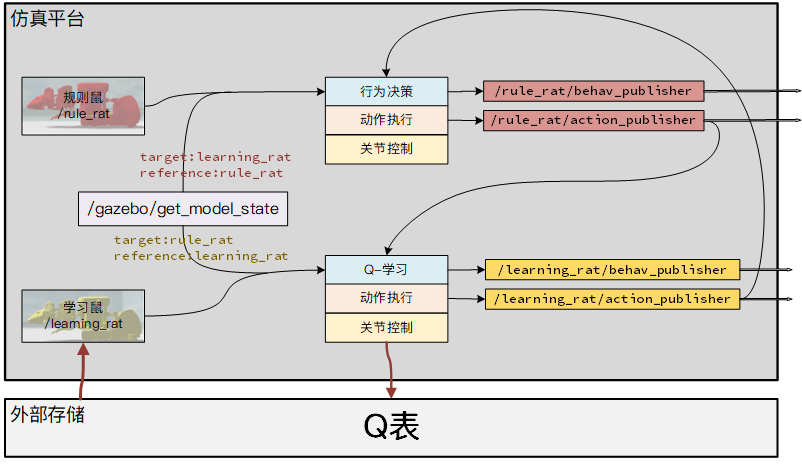
\includegraphics[height=8cm]{images/ch04/learning.png}
%  \caption{机器鼠行为交互仿真实验资源}\label{figure_resource}
%\end{figure}

在实验进行时,用户无需进行额外操作。为提高仿真系统的稳定性,同时保证系统在受到内外干扰终止运行后能保留已学习的知识,以便重启时能继续学习,学习鼠在每一轮学习完成后均会向磁盘内文件写入Q表数值,当系统启动运行时会读取该文件。
\subsection{数据收集}
ROS系统具备存储日志的功能,各日志文件以节点区分存储。除此以外,所搭建的仿真平台提供了发布学习鼠和规则鼠行为、动作的节点,利用rosbag可以存储这些节点发布的消息。同时,利用录屏软件获得学习鼠训练过程中的表现作为直观验证方式。
